\chapter{Captura de requisitos}
%\newpage
%Que tiene que cumplir el trabajo que se va a desarrollar, 
%que necesidades tiene que satisfacer, quienes van a ser sus usuarios, etc.
%
%En un trabajo de desarrollo de software tradicional se 
%documentará mediante el Modelo de casos de uso y la jerarquía 
%de actores, acompañando cada caso de uso y cada actor de una pequeña definición.

\section{Diagrama de casos de uso}
En el diagrama de casos de uso, se puede ver que acciones puede realizar el usuario en cualquier momento, y cuales
est\'an supeditadas a ciertas condiciones. N\'otese que las condiciones de los ``extend" \ son los comentarios a\~nadidos
a los subcasos de uso.

\begin{figure}[h]
\centering
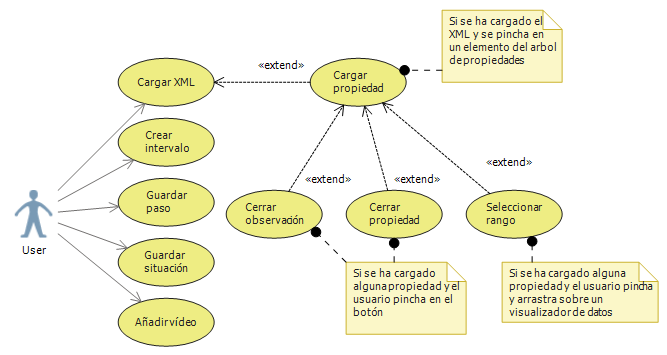
\includegraphics[width=1.0\linewidth]{./Figures/useCaseDiagram.png}
\caption[Diagrama de casos de uso]{Diagrama de casos de uso}
\label{fig:useCaseDiagram}
\end{figure}


\section{Modelo de dominio}
Los datos que se guardan son ciertamente bastante simples, ya que para la tripleta Instante, Observaci\'on y Propiedad,
toma un \'unico valor posible. 

La Figura \ref{fig:ModelodeDominio} representa tanto los datos de entrada del software, tanto los datos
de salida.

\begin{figure}[H]
\centering
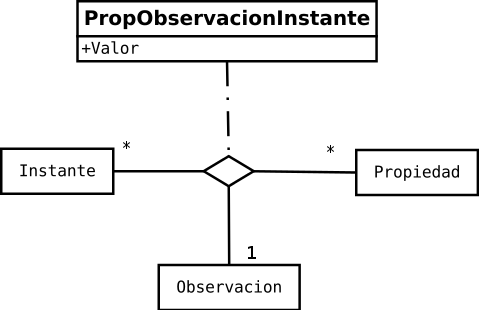
\includegraphics[width=0.7\linewidth]{./Figures/ModelodeDominio}
\caption[Modelo de dominio]{Modelo de dominio}
\label{fig:ModelodeDominio}
\end{figure}
